\documentclass[12pt]{article}
\usepackage[utf8]{inputenc}
\usepackage[T1]{fontenc}
\usepackage{lmodern}
\usepackage{graphicx}
\usepackage{subcaption}
\usepackage{listings}
\usepackage{color}
\usepackage[svgnames]{xcolor}
\usepackage[a4paper,bindingoffset=0.2in,%
left=1in,right=1in,top=1.5in,bottom=1.5in,%
footskip=.25in]{geometry}

\definecolor{dkgreen}{rgb}{0,0.6,0}
\definecolor{gray}{rgb}{0.5,0.5,0.5}
\definecolor{mauve}{rgb}{0.58,0,0.82}

\lstset{frame=tb,
	language=Python,
	aboveskip=3mm,
	belowskip=3mm,
	showstringspaces=false,
	columns=flexible,
	basicstyle={\small\ttfamily},
	numbers=none,
	numberstyle=\tiny\color{gray},
	keywordstyle=\color{blue},
	commentstyle=\color{dkgreen},
	stringstyle=\color{mauve},
	breaklines=true,
	breakatwhitespace=true,
	tabsize=3,
	extendedchars=true,
	literate={ą}{{\k a}}1 {ę}{{\k e}}1 {ś}{{\'s}}1 {ć}{{\'c}}1 {ź}{{\'z}}1 {ż}{{\. z}}1 {ń}{{\'n}}1 {ł}{{\l}}1 {ó}{{\'o}}1,
}

\pagenumbering{gobble}
\graphicspath{{./zdjs/}}


\begin{document}
\title{Sprawozdanie - Odtwarzanie muzyki z nut na pięciolinii}
\author{Marcin Zatorski 136834, Sebastian Michoń 136770}
\date{\vspace{-2ex}}
\maketitle

\section{Cel i zakres projektu}
Celem projektu było zaimplementowanie aplikacji odczytującej nuty z obrazu z kamery, a następnie odtworzenie ich za pomocą głośnika z użyciem płytki Raspberry Pi.

\section{Schemat, Idea}
\subsection{Idea wykrywania nut}
\begin{enumerate}
	\item 
\end{enumerate}

\subsection{Schemat}
\begin{figure}[h!]
	\centering
	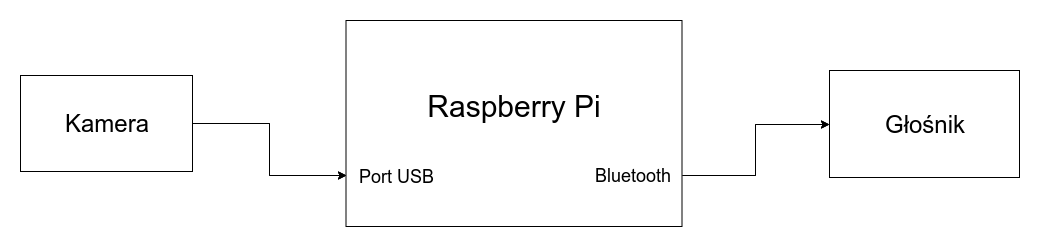
\includegraphics[width=0.9\linewidth]{SW-schematic.png}
	\caption{Schemat połączeń}
	\label{fig:schemat}
\end{figure}
	
\section{Projekt a realizacja}
Aplikacja została napisana w języku Python i Cython. Rozpoznawanie nut zostało zaimplementowane przy użyciu biblioteki OpenCV. Aplikacja jest w stanie rozpoznać nuty z wysoką skutecznością, o ile zdjęcie zostało zrobione w dobrych warunkach oświetleniowych. Algorytm rozpoznaje tylko część symboli - nuty (całe nuty, półnuty, ćwierćnuty i ósemki) oraz klucze. Tą część algorytmu można by rozszerzyć o rozpoznawanie większej ilości symboli. Dokładność rozpoznawania nut również można by ulepszyć na przykład poprzez zastosowanie metod maszynowego uczenia.
	
W trakcie rozwijania projektu dużą przeszkodą była szybkość działania. Dzięki przepisaniu części kodu do języka Cython oraz optymalizacjom aplikacja działa zadowalająco szybko.
	
Pierwotnie w projekcie zakładaliśmy użycie płytki BeagleBone Black. Zdecydowaliśmy się jednak na użycie płytki Raspberry Pi - umożliwiło to proste podłączenie głośnika przez Bluetooth.
	
Aplikacja nie pozwala na wybranie dźwięku instrumentu, co było początkowo planowane. Aplikacja odtwarza jednocześnie nuty tylko z jednej pięciolinii, a nie z obu.

Aplikację można by rozwinąć o lepszy interfejs użytkownika. Obecnie aplikacja jest uruchamiana z linii poleceń. Warto by było dodać na przykład GUI pokazujące obraz z kamery lub przycisk umożliwiający wykonanie zdjęcia.
Aplikacja nie pozwala na wybranie dźwięku instrumentu, co było początkowo planowane. Aplikacja nie odtwarza nut z obu pięciolinii jednocześnie - są odtwarzane po kolei.
	
Aplikację można rozwinąć o lepszy interfejs użytkownika. Obecnie aplikacja jest uruchamiana z linii poleceń. Warto dodać na przykład GUI pokazujące obraz z kamery lub przycisk umożliwiający wykonanie zdjęcia. Brak interfejsu utrudnia ocenę, czy aplikacja działa poprawnie.

\section{Kluczowe fragmenty kodu}
\begin{lstlisting}[language=Python]
#Binaryzacja obrazka - przyjmuje jako input obraz w odcieniach szarości, zwraca obraz czarno biały z uwypuklonymi ciemniejszymi niż tło obszarami. Opiera się na kompletnym zaciemnieniu obszarów, wokół których kolor nigdy się nie zmienia i standardowej binaryzacji dla pozostałych obszarów obrazka
def binarization(bwimg):
	edges = cv.Canny(bwimg,50,150,apertureSize = 3)
	edges2=cv.filter2D(bwimg, -1, kernel[1])
	edges2=cv.Canny(edges2,50,150,apertureSize = 3)
	bwimg=cv.adaptiveThreshold(bwimg, 255, cv.ADAPTIVE_THRESH_GAUSSIAN_C, cv.THRESH_BINARY, Hypers['Binarization_conn'], 1)
	###i wiele linii więcej
	return bwimg
	

#Rotacja obrazka - przyjmuje obraz przed i po binaryzacji, znajduje długie linie na oryginalnym obrazku po czym dzeli je na klasy abstrakcji tak, że linie x, y są w 1 klasie abstrakcji, jeśli istnieje takie z, że z*0.01<=cos(x),cos(y)<z*0.01+0.01. W zależności od klasy abstrakcji o największej mocy zbioru ustawiam obrazek tak, aby jak najwięcej linii było poziomych. Zwraca Obrócone obrazy - oryginalny i zbinaryzowany
def rotate_image(img, fimg):
	img2=fimg.copy()
	edges = cv.Canny(img2,50,150,apertureSize = 3)
	lines = cv.HoughLinesP(edges,1,np.pi/180,100,100,10)
	###i wiele linii więcej
	rotated_mat = cv.warpAffine(img, rotation_mat, (bound_w, bound_h), borderValue=255)
	rotated_org = cv.warpAffine(fimg, rotation_mat, (bound_w, bound_h), borderValue=255)
	return rotated_mat, rotated_org
	
#Usuwanie linii - przyjmuje poddany rotacji zbinaryzowany obraz, zwraca zbinaryzowany obraz pozbawiony linii przez referencję, a także miejsca występowania pięciolinii. Kod opiera się na kilkudziesięciu heurystykach grafowych (obrazek jest traktowany jako graf, który można przejść algorytmem Breadth First Search zatrzymując algrytm po znalezieniu wszystkich linii poziomych). Algorytm celem skrócenia czasu jego wykonania został przeniesiony do Cythona
def findlinez(unsigned char[:,:] bwimg, shp):
	#Warto zwrócić uwagę na składnię, w szczególności przyspieszanie kodu za pomocą memoryviewa
	cdef int skv=2, y=1, kk=1, iF=0, jF=1, deadl=0, deadr=1, highx, lowx, x1, x2, C=140000, myconst=Hyperparameters['Upgrade']
	cdef int lenpath=0, lp2=0, D=3000
	solution=[]
	cdef unsigned char[:,:] check=np.zeros((bwimg.shape[0], bwimg.shape[1]), dtype='uint8')
	cdef int[:] par=np.zeros((C), dtype='int32')
	cdef int[:] miss=np.zeros((C), dtype='int32')
	cdef int[:] w=np.zeros((C), dtype='int32')
	###Cała ta heurystyka ma dalej około 300 linijek...
	return solution

#Znajdowanie pięciolinii wśród usuniętych linii - przyjmuje obrazek z usuniętymi liniami(img) i ich miejscami w obrazku(sol), zwraca miejsca występowania pięciolinii i ich parametry - szczególności wysokość pięciolinii i grubość linii, korzystając między innymi ze struktury zbiorów rozłącznych.
def line5finder(sol, img):
	dp=[0]*len(sol)
	kenose=[0]*len(sol)
	tv=[0]*len(sol)
	dtrl, dtrr=Hypers['Dt']
	for i, x in enumerate(sol):
		make_set(i)
		if (i>0):
			dp[i]=sol[i][0]-sol[i-1][0]
			tv[i]=i
	##Kildziesiąt linii dalej...
	return wynne
	
	
#Kluczowa część usuwania linii - kod przetwarzający obrazek od początku, zwracający obrazek z usuniętymi liniami.
def remove_staff_lines(input_img):
	imgb=input_img.copy()
	shorig=imgb.shape
	
	###Binaryzacja obrazka
	imv=binarization(imgb.copy())
	###Rotacja obrazka
	img2, img_original =rotate_image(imv, imgb)
	img2=cv.adaptiveThreshold(img2, 255, cv.ADAPTIVE_THRESH_GAUSSIAN_C, cv.THRESH_BINARY, Hypers['Binarization_conn'], 1)
	#Obramowanie obrazka w 10 czarnych linii z każdej strony - ułatwia dalsze przetwarzanie
	ss=np.zeros((img2.shape[0]+20, img2.shape[1]+20), dtype=str(img2.dtype))
	ss[10:-10,10:-10]=img2
	img2=ss.copy()
	
	# Padding oryginalnego obrazka
	padded = np.zeros((img_original.shape[0]+20, img_original.shape[1]+20), dtype=str(img_original.dtype))
	padded[10:-10,10:-10] = img_original
	
	###Usuwanie linii poziomych
	sol=findlinez(img2, shorig)
	###Znajdywanie pięciolinii 
	wynne=line5finder(sol, img2)
	#Zwracanie obrazka po procesie, oryginalnego obrazka z paddingiem i parametrów pięciolinii
	return ~img2, padded, wynne


\end{lstlisting}

\section{Zdjęcia fizycznych połączeń urządzeń}
\begin{figure}[h!]
	\centering
	\begin{subfigure}[b]{0.32\linewidth}
		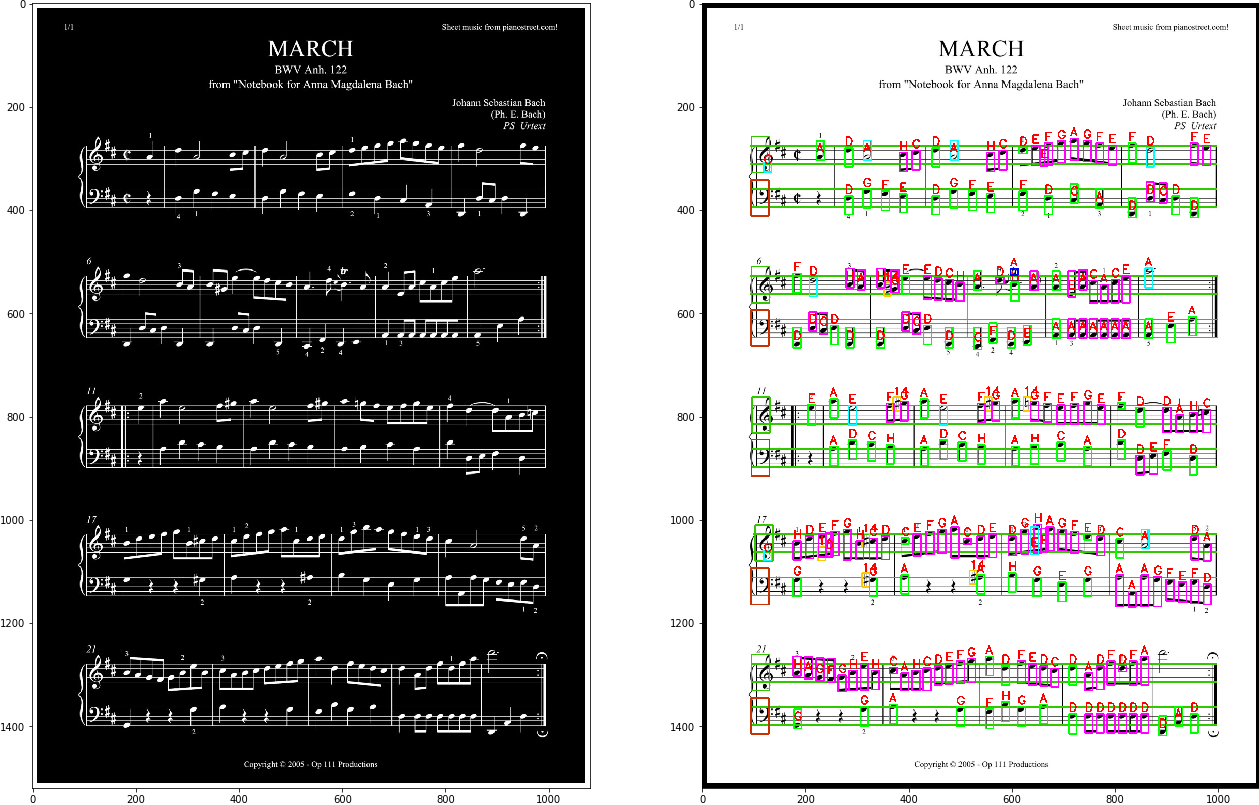
\includegraphics[width=\linewidth]{Zdj0.png}
		\caption{Pierwszy podpis}
	\end{subfigure}
	\begin{subfigure}[b]{0.32\linewidth}
		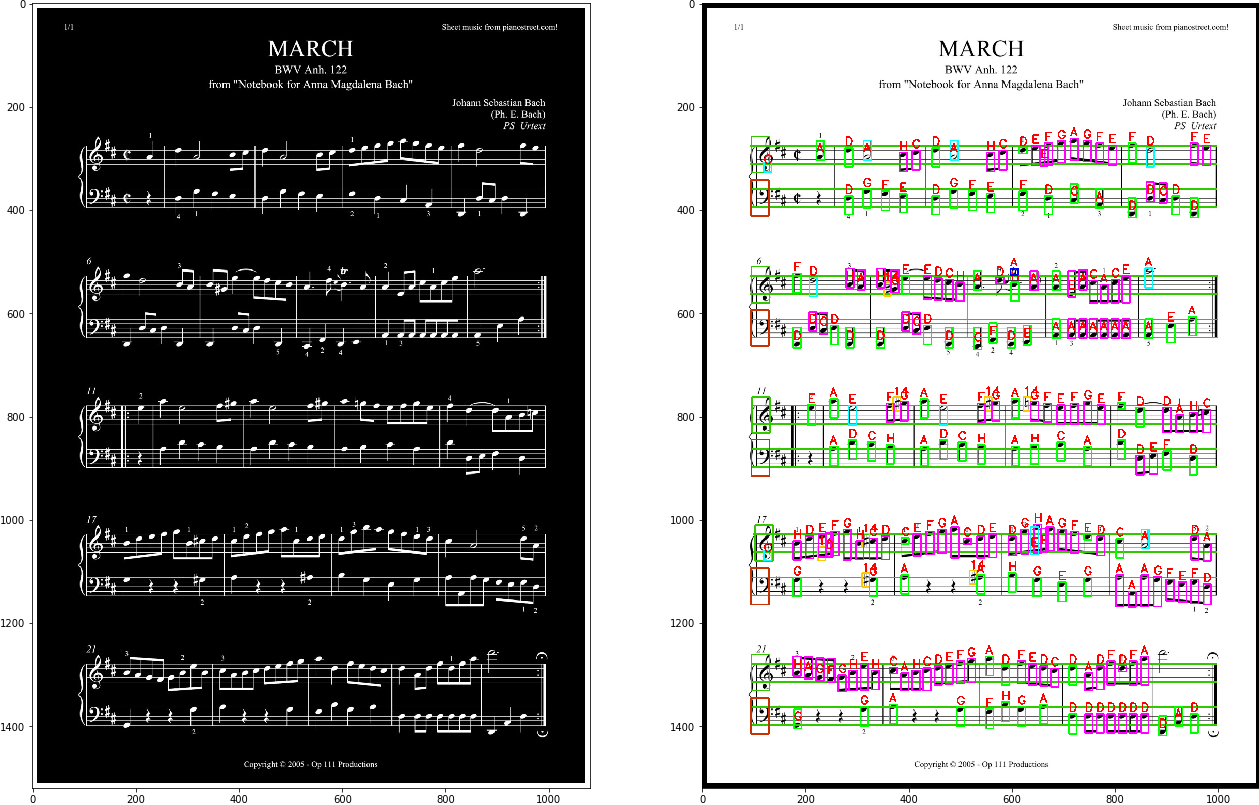
\includegraphics[width=\linewidth]{Zdj0.png}
		\caption{Drugi podpis}
	\end{subfigure}
	\begin{subfigure}[b]{0.32\linewidth}
		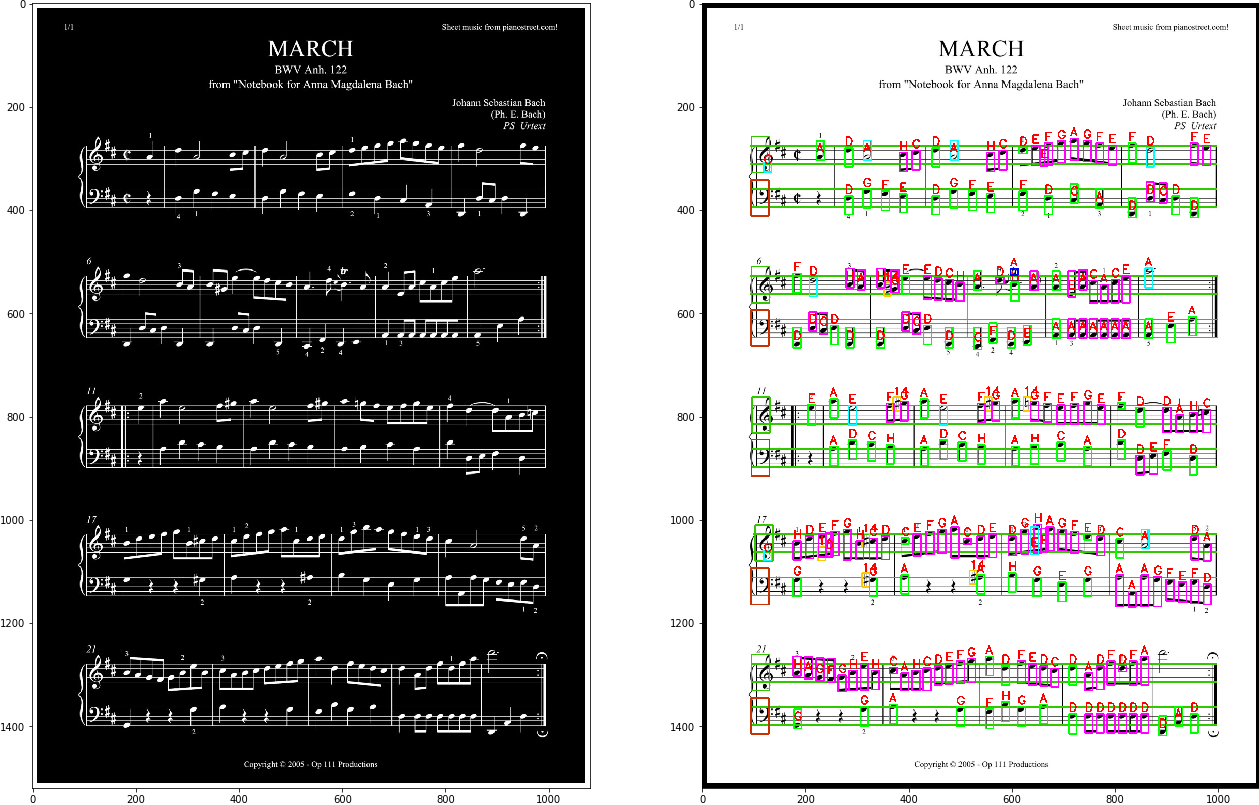
\includegraphics[width=\linewidth]{Zdj0.png}
		\caption{Trzeci podpis}
	\end{subfigure}
	
	\begin{subfigure}[b]{0.48\linewidth}
		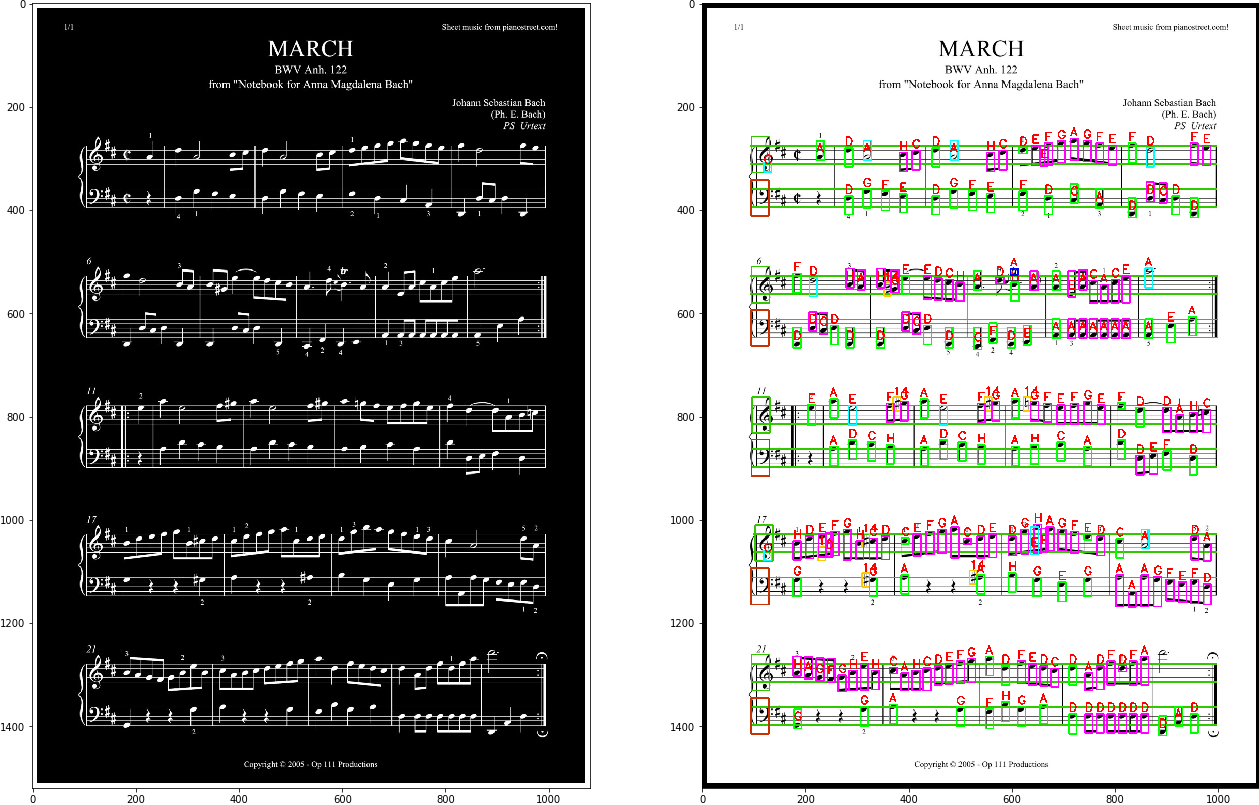
\includegraphics[width=\linewidth]{Zdj0.png}
		\caption{Czwarty podpis}
	\end{subfigure}
	\begin{subfigure}[b]{0.48\linewidth}
		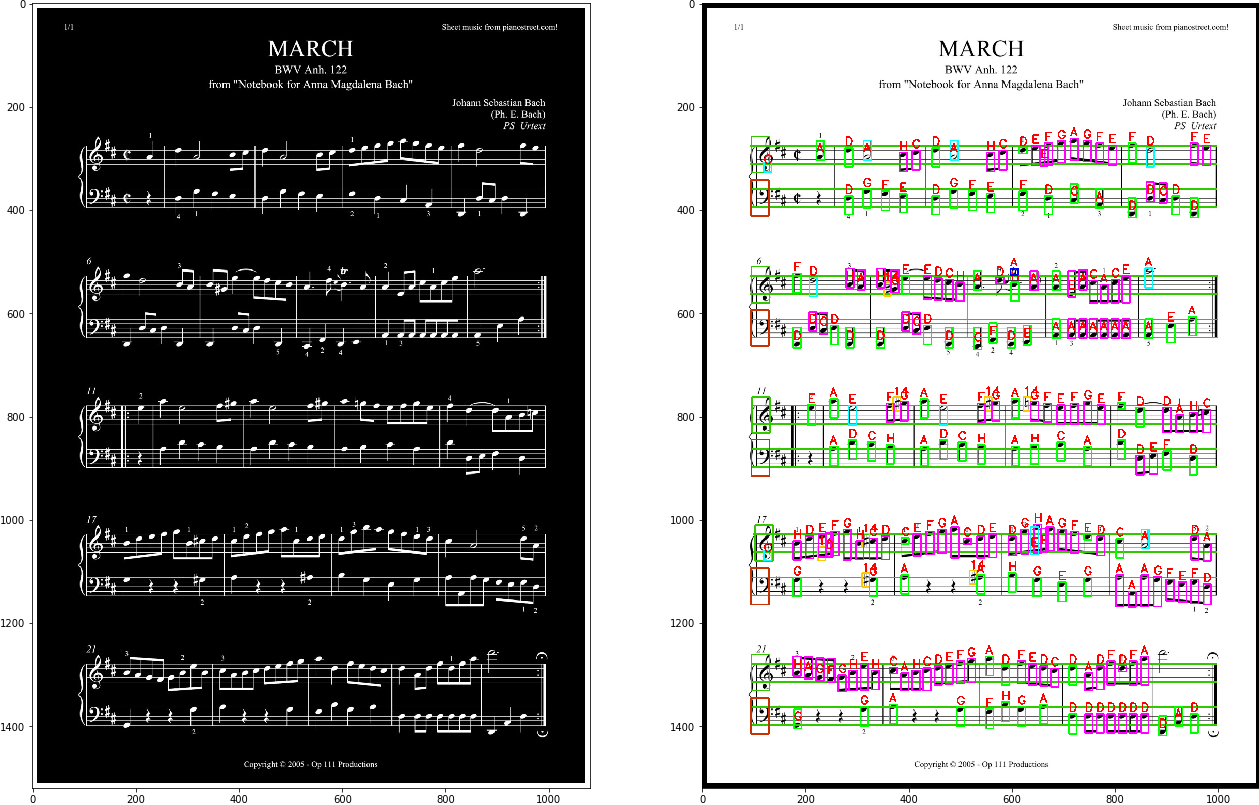
\includegraphics[width=\linewidth]{Zdj0.png}
		\caption{Piąty podpis}
	\end{subfigure}
\end{figure}

\section{Podsumowanie, wnioski}
Aplikacja realizuje swój cel, choć są elementy które można poprawić lub które nie zostały zaimplementowane. Użyty przez nas algorytm uzyskuje wysoką skuteczność przy dobrej jakości zdjęcia; zasadna byłaby próba ulepszenia kodu poprzez użycie metod adaptatywnych, opartych na funkcji kosztu zamiast metod analitycznych przetwarzania obrazu.

\end{document}
